\documentclass[12pt,a4paper,UTF8]{ctexart}




%设置页边距
\usepackage{geometry}
\geometry{left=2.5cm,right=2.5cm,top=2.5cm,bottom=2.5cm}




%需要用到的扩展包
\usepackage{xeCJK,amsmath,paralist,enumerate,booktabs,multirow,graphicx,float,subfig,setspace,listings,lastpage,hyperref}
\usepackage{fancyhdr}




%设置页眉页脚以及页码
\pagestyle{fancy}
\rhead{伏安法测定电阻}
\lhead{大学基础物理实验报告}
\cfoot{Page\thepage/\pageref{LastPage}}
\rfoot{\today}




%报告中用到的图片存放在这个tex文件所在目录中的figures子目录中
\graphicspath{{figures/}}









%报告开始
\begin{document}
	
	
	
	
	%设置课程标题
	\begin{center}
		\heiti\LARGE{《大学基础物理实验》课程实验报告}
	\end{center}
	
	
	
	
	%设置实验人信息以及实验时间表格


		\begin{center}
			\begin{tabular}{lcr}
				
				{\songti 姓名及学号:蒋丰毅2211082}  \quad 专业:工科试验班 \quad 年级:22级 \quad 座号:10\\
				{\songti  学院:软件学院 \quad 实验组别:C组\quad 实验时间:2023年3月24日~星期五~上午}\\
				
				
			\end{tabular}
		\end{center}
	\vspace{-0.2cm}
	{\noindent}	 \rule[-10pt]{17.5cm}{0.05em}\\

	\vspace{-0.4cm}
	
	
	
	
	
	
	%实验题目
	\begin{center}
		\LARGE\textbf{伏安法测定电阻}
	\end{center}
	

	
	%实验原理
	\subsection*{[实验原理]}
	\subsubsection*{线性元件和非线性元件}
	\par 伏安特性曲线是以电流$U$为横坐标,电压$I$为纵坐标作出的I-U图。通常情况下,导电金属丝,碳膜电阻,金属膜电阻等的伏安特性曲线是一条直线,称其为线性元件;二极管等元件的伏安特性曲线不是一条直线,这类元件称为非线性元件。
	\vspace{0.2cm}
	\begin{figure}[htbp]
		\centering
		\begin{minipage}[t]{0.48\textwidth}
			\centering
			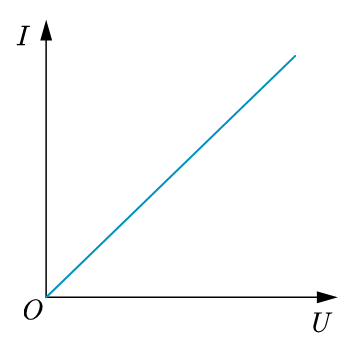
\includegraphics[width=5cm]{线性元件}
			\caption{线性元件}
		\end{minipage}
		\begin{minipage}[t]{0.48\textwidth}
			\centering
			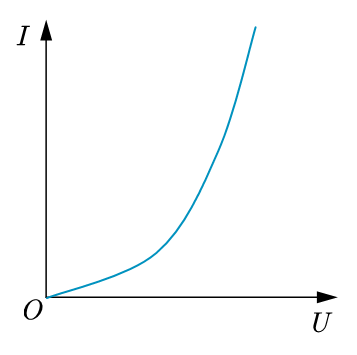
\includegraphics[width=5cm]{非线性元件}
			\caption{非线性元件}
		\end{minipage}
	\end{figure}
	\vspace{-0.8cm}
	\subsubsection*{测量电路}
	\par 本实验中测量电路分为两种:分压式和限流式,本次实验选择分压电路,电压表内接
		\begin{figure}[htbp]
		\centering
		\begin{minipage}[t]{0.48\textwidth}
			\centering
			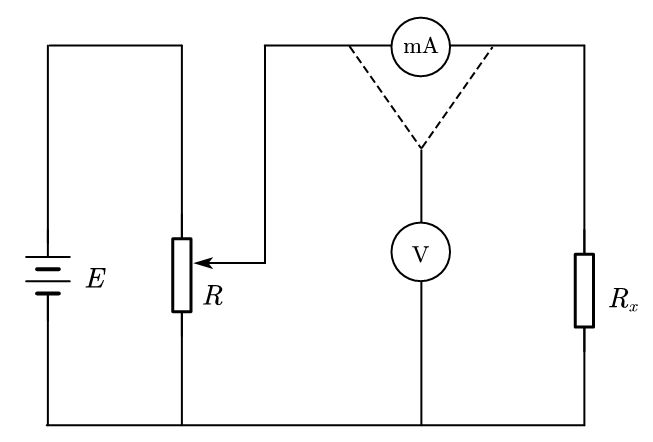
\includegraphics[width=6cm]{分压电路}
			\caption*{(a)分压电路}
		\end{minipage}
		\begin{minipage}[t]{0.48\textwidth}
			\centering
			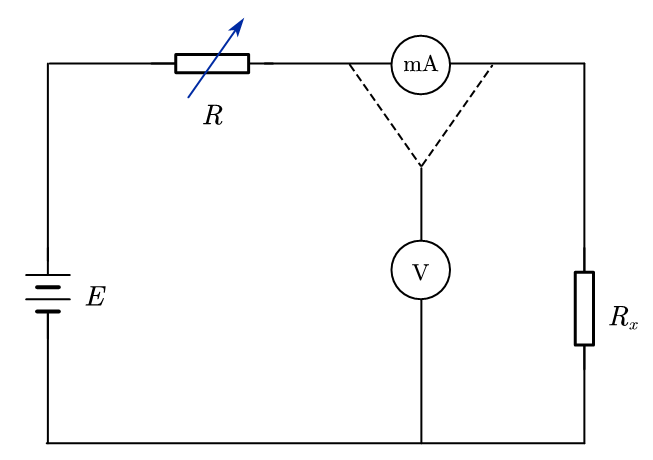
\includegraphics[width=6cm]{限流电路}
			\caption*{(b)限流电路}
		\end{minipage}
	\caption{测量电路选取}
	\end{figure}
	
	

	
	\subsection*{[实验仪器和万用表测量数据]}
	\par 直流稳压电源
	\par 台式万用表:GDM8342
	\par 手持万用表:VT61B
	\par 金属膜电阻$R_x$阻值:110$\Omega$
	\par 直流稳压电源输出电压:1.47$V$
	\par 二极管$PN$结电压:0.386mV

	
	
	
	
	
	
	
	
	%实验内容与分析
	\subsection*{[测量数据]}
	\par 实验测量数据如下
	\begin{table}[!h]
		\centering
		\begin{tabular}{|l|l|l|l|l|l|l|l|l|l|}
			\hline
			$U(V)$ & 0.046 & 0.099 & 0.154 & 0.217 & 0.259 & 0.316 & 0.373 & 0.416 & 0.441 \\ \hline
			$I(mA)$ & 0.41   & 0.90   & 1.39   & 1.96    & 2.34    & 2.85   & 3.37  & 3.75    & 3.98  \\ \hline
		\end{tabular}
		\caption{金属膜伏安特性曲线原始数据表}
	\end{table}

	\begin{table}[!h]
		\centering
		\begin{tabular}{|l|l|l|l|l|l|l|l|l|l|}
			\hline
			$U(V)$ & 0.412 & 0.591 & 0.618 & 0.65 & 0.670 & 0.682 & 0.694 & 0.710  & 0.740 \\ \hline
			$I(mA)$ & 0.02   & 2.22  & 3.48   & 5.60  & 7.48   & 8.86  & 10.20  & 12.71 & 18.20 \\ \hline
		\end{tabular}
		\caption{二极管正向伏安特性曲线原始数据表}
	\end{table}
	\vspace*{-0.6cm}
	\subsection*{[数据处理]}
			\begin{figure}[h!tbp]
		\centering
		\begin{minipage}[t]{0.48\textwidth}
			\centering
			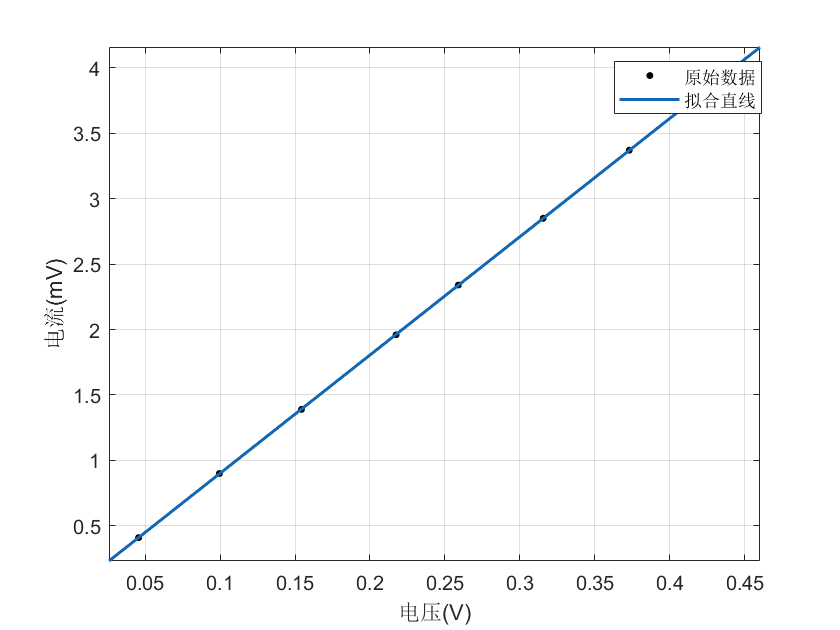
\includegraphics[width=7cm]{线性电阻图片}
			\caption*{线性电阻直线拟合}
		\end{minipage}
		\begin{minipage}[t]{0.48\textwidth}
			\centering
			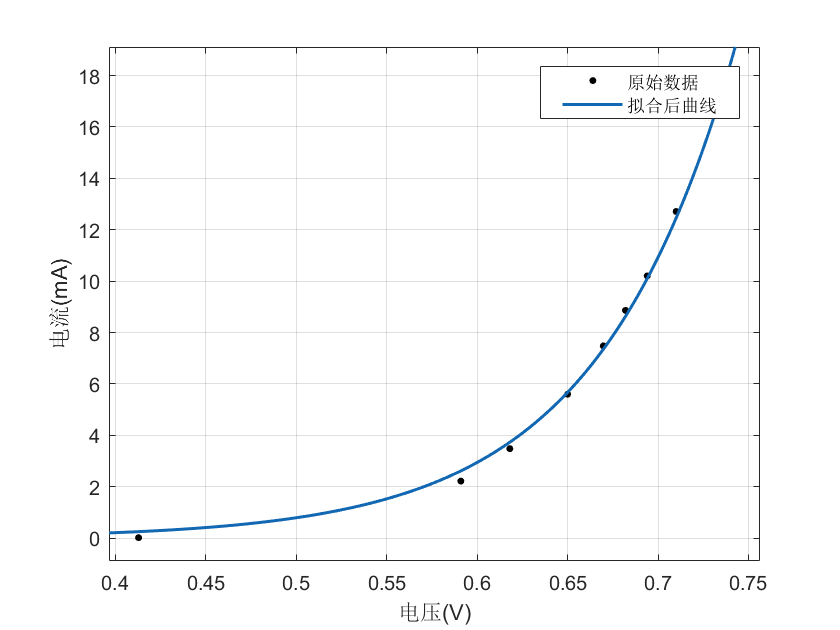
\includegraphics[width=7cm]{非线性电阻图片}
			\caption*{非线性电阻曲线拟合}
		\end{minipage}
		\caption{实验数据处理}
	\end{figure}
	\par 对于线性元件,Matlab拟合直线的结果为$y = 9.035x-0.00101737$,选取较远的两个点,带入公式
	\[\overline{R_x}=\frac{U_2-U_1}{I_2-I_1-\dfrac{U_2-U_1}{R_V}}
	\]
	\clearpage
	\par 计算得$\overline{R}_x=\dfrac{1}{9.035-\dfrac{1}{10^7}}\times1000\approx110.7\Omega$
	\par 在直线上选取两个足够远的点$(0.01,0.0893)$和$(0.50,4.5165)$计算:
	\[\Delta U = \pm 0.0002*0.441+4*0.0001 = \pm 0.00048\]
	\[\Delta I = \pm 0.012*3.98+3*0.01 = \pm 0.78\]
	\par 计算相对误差$\rho_x$
	\[\rho_x=\sqrt{\rho_V^2+\rho_z^2}=\sqrt{\left(\frac{\Delta U}{U_2-U_1}\right)^2+\left(\frac{\Delta L}{I_2-I_1}\right)^2}=0.0775\]
	\par 则误差为$\Delta R = \overline{R}_x\times \rho_x = 8.57\Omega$,求得最终结果为
	\[R_x = (110.7\pm 8.6)\Omega \]
	\subsubsection*{二极管数据处理}
	\par 从图中可以看出
	\par 在2.00mA下的阻值为$\frac{0.62}{2}*1000 = 31\Omega$
	\par 在8.00mA下的阻值为$\frac{0.68}{8}*1000 = 85\Omega$
	\subsection*{思考题}
	

			\begin{figure}[htbp]
		\centering
		\begin{minipage}[t]{0.48\textwidth}
			\centering
			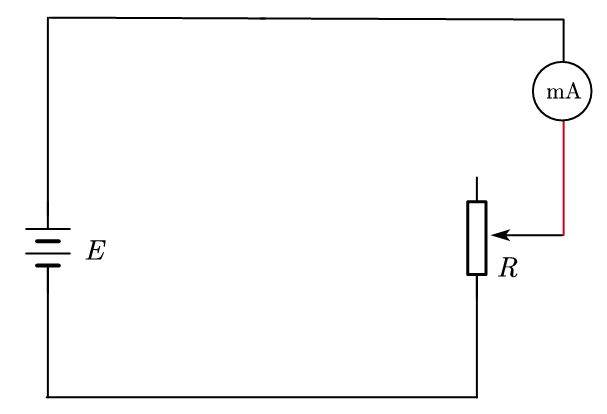
\includegraphics[width=4cm]{思考题1}
			\caption*{第一次测量}
		\end{minipage}
		\begin{minipage}[t]{0.48\textwidth}
			\centering
			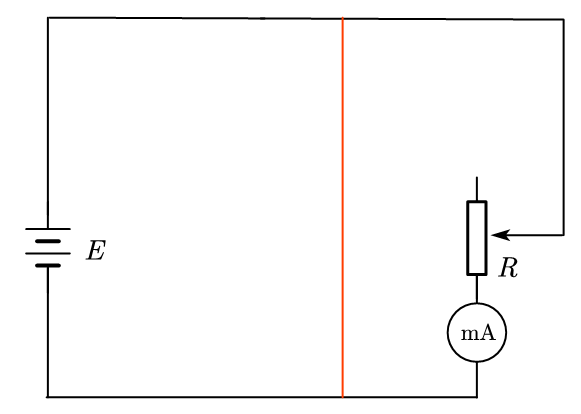
\includegraphics[width=4cm]{思考题2}
			\caption*{第二次测量}
		\end{minipage}	\begin{minipage}[t]{0.48\textwidth}
		\centering
		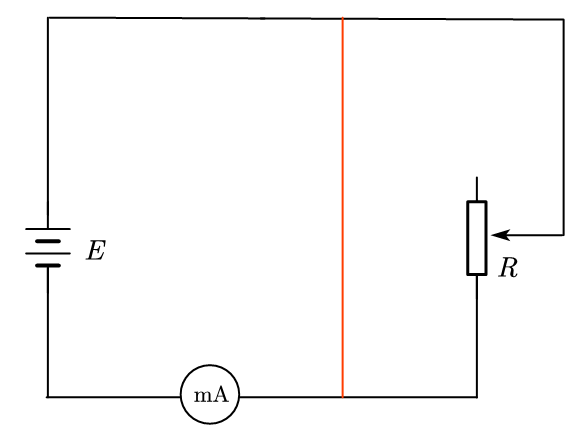
\includegraphics[width=4cm]{思考题3}
		\caption*{第三次测量}
	\end{minipage}
		\caption{测量电路}
	\end{figure}
	\par 注意,三次测量保证滑动变阻器都在同一个位置。可以列出方程组
	$$
	\begin{cases}
		E = I_{测1}(R_A+R+R_x)\\
		E = I_{测2}(R+R_A)\\
		E = I_{测3}(R_A+\frac{R_xR}{R_x+R})
	\end{cases}
	$$	
	\par 方程有三个未知数,故可以解得$R_x$
	
	
	
	
	


\end{document}
